\subsection{Experiment 1 Quantitative Analysis Results} \label{results-1-quan}
In this section, we will first present descriptive statistics of the raw data in our first experiment. Then, we will explain our feature engineering and data transformation process based on the raw data. Lastly, we will introduce the Bayesian Model we applied in our analysis and present the analysis results.

\subsubsection{Descriptive Statistics of the Raw Data}
% -- raw data
%     describe the dataset, total # of participants in each group before and after dataset cleaning, demographics of each group;
    
Overall, we collected 223 complete responses in the first experiment. We removed 4 responses after checking the quality of the responses due to reasons such as not answering the qualitative question seriously or misunderstanding the prompt. Among the 219 remaining responses, 56 completed the Likert path, and the rest were distributed relatively evenly across the remaining 6 paths with various orders of QV, ranging from 24 to 28 responses per path. Aggregating responses from all 6 paths, the number of responses we got for QV with 36 credits (QV36), QV with 108 credits (QV108) and QV with 324 credits (QV324) were 107, 108, and 111 respectively. (To-do: maybe add a hierarchical graph the represents how responses from different paths are aggregated)

We recruited the participants with the goal of constructing a sample that was representative of the US census data in terms of age and education level. Having a representative sample is in particularly critical in our study because these voting and survey tools should aim to be designed for the general population. Based on Table \ref{fig:demo_exp1}, all the groups closely followed the demographics of the US population in both age and education level. This ensured that our results were not biased to a certain subgroup of the population, which is generally hard to achieve in MTurk studies without specific control. 

\begin{figure}[htpb]
    \centering
    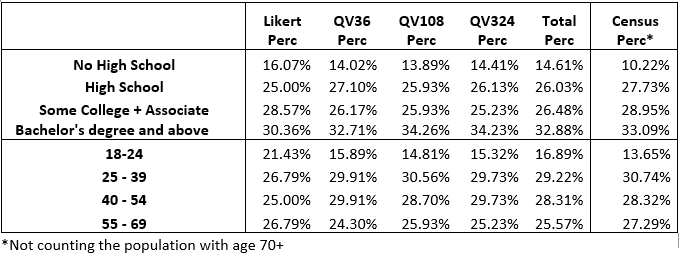
\includegraphics[width=0.7\textwidth, keepaspectratio=true]{content/image/demographics_table.png}
    \caption{
        Sample Demographics Statistics Compared to US Census Data (Will fix into a table later)
    }
    \Description[Sample Demographics Statistics Compared to US Census Data for experiment 1]{Sample Demographics Statistics Compared to US Census Data for experiment 1}
    \label{fig:demo_exp1}
\end{figure}
    
%     donation descriptive statistics: perc of non-zero donation, total donation amount comparison across groups, donation distribution across topics between groups

In this experiment, each set of survey responses by a participant in a condition could be matched to the set of donation decisions made by the same participant. Since we would like to use the donation outcome of a participant as a proxy of his/her true preferences across the nine charity topics, we could only do so with participants that donated a non-zero amount of money. Therefore, we further filtered the dataset to keep only the responses that had a non-zero total donation amount. Across all the conditions, the average non-zero donation rate was 73.3\%, consistent with the results provided by Fehr and Gintis in 2007 \cite{fehr2007human}, which suggested that about 30\% of the population would always free-ride in public goods provision regardless of what others do. The donation rate in each condition closely centered around the average donation rate, ranging from 70.37\% (in QV108) and 77.19\% (in Likert). The number of valid responses after this step for Likert, QV36, QV108, and QV324 were 44, 76, 76 and 84 respectively.

Among those who donated a non-zero amount, participants exhibited different behaviors when deciding how much to donate in total. As shown in Figure \ref{fig:total_don_exp1}, there were two main clusters for the total donation amount. The first cluster centered around \$9-12 and most data points in this cluster lied within the range of \$5 to \$20. This group of people, making up about 60\% of the entire sample, donated part of the lottery winning amount but still kept a significant portion for themselves. The second cluster was between \$33 to \$35, suggesting that this group of people chose to contribute almost the full amount of the lottery prize. There were approximately 25\% of the participants who behaved this way. In most cases, the distribution pattern across conditions were relatively consistent, except that there were almost twice the proportion of participants in the Likert condition that donated almost the full amount compared to the other QV conditions. One possible explanation for the difference would be that the amount of effort required to complete the Likert condition was much lower than that of QV, and participants felt less tempted to earn extra reward for their time spent in the Likert condition. Overall, we found that the total amount of donation per participant was large enough to be distributed across charities in a way that could represent the full picture of his/her underlying true preferences for nine topics.

\begin{figure}[htpb]
    \centering
    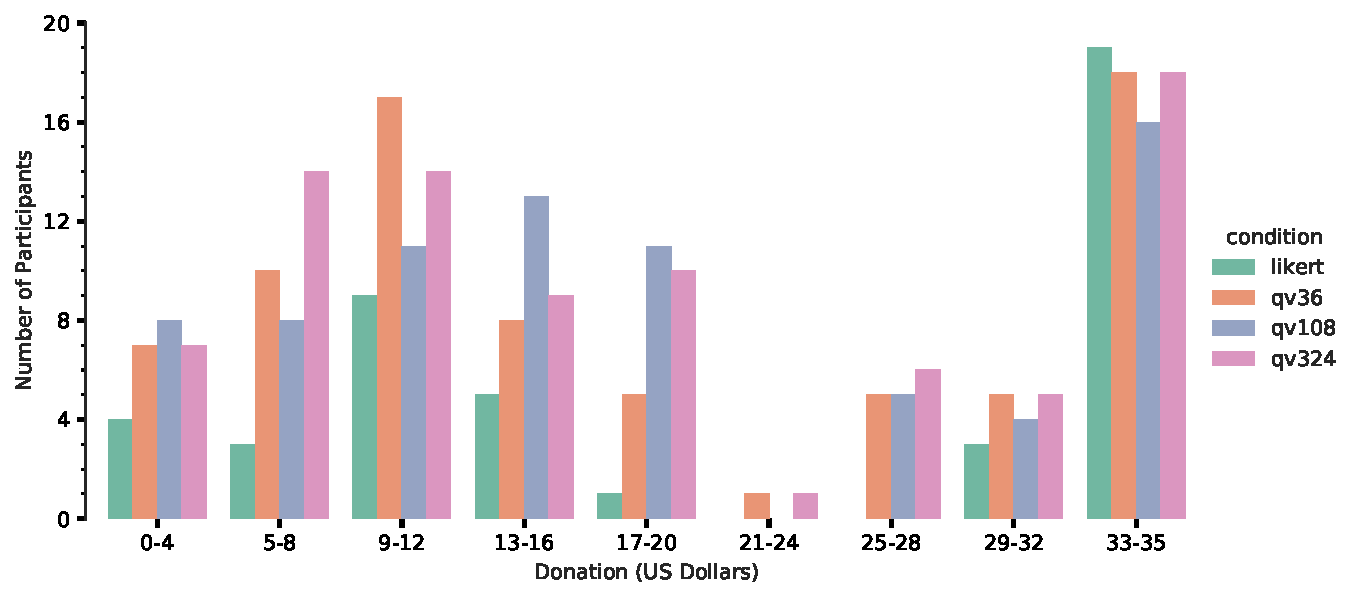
\includegraphics[width=0.8\textwidth, keepaspectratio=true]{content/image/total_contributions_across_conditions.pdf}
    \caption{
       Distributions of Total Donation Amounts across Conditions
    }
    \Description[Distributions of Total Donation Amounts across Groups for experiment 1]{Distributions of Total Donation Amounts across Groups for experiment 1}
    \label{fig:total_don_exp1}
\end{figure}

Given the aggregated total donation amount across all the participants in each condition, the amount was distributed to the nine charities in a highly varying manner as shown in Figure \ref{fig:topic_don_exp1}. The environment-related, health-related, and human-related charities were consistently the most popular ones among all the options in different groups, while the art-related, international-related, and faith-related ones were always the least popular. However, we could see some differences in the population-level preferences towards charities across the four conditions. For example, the pets-related charity received far less donation in percentage than the three QV groups. This suggested that there was a good amount of variance in people's opinions towards the nine topics, making the surveying task meaningful.

\begin{figure}[htpb]
    \centering
    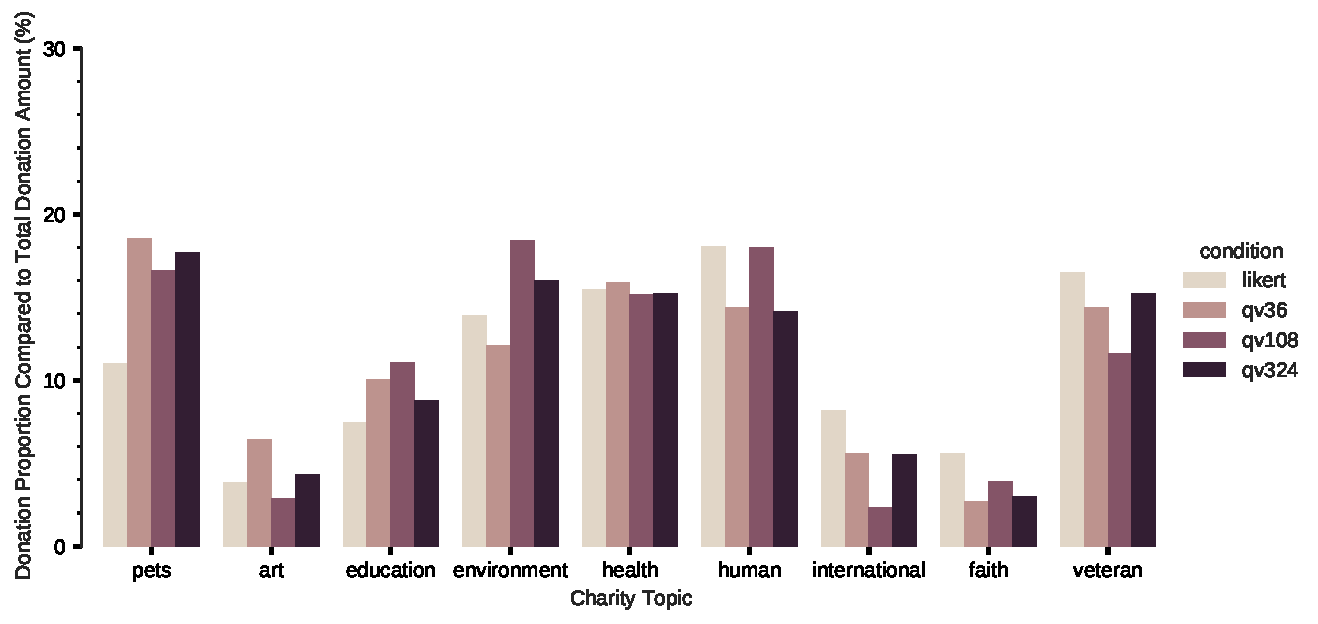
\includegraphics[width=0.8\textwidth, keepaspectratio=true]{content/image/normalized_contributions_per_topic_across_conditions.pdf}
    \caption{
      Percentage Contribution Amount per Topic with Respect to the Total Donation Amount across Conditions
    }
    \Description[Percentage Contribution Amount per Topic with Respect to the Total Donation Amount across Conditions for experiment 1]{Percentage Contribution Amount per Topic with Respect to the Total Donation Amount across Conditions for experiment 1}
    \label{fig:topic_don_exp1}
\end{figure}

%     QV & Likert votes descriptive statistics: votes distribution per topic across groups, budget usage distribution across QV groups


    
% -- data transformation to alignment measurement
%     describe the calculation of cosine similarity angle theta
%     mention our test of checking if other factors impact total donation amount -> absolute vs. normalized donation amount
%     show histogram and other descriptive statistics of the angle data
    
% -- Bayesian formulation
%     why Bayesian
%     the type of analysis question
%     choice of the likelihood function
%     choice of prior distributions
    
% -- Results analysis
%     Tools: PyMC3, MCMC, NUTS
%     Describe fitted values & convergence (trace plots)
%     Describe effect size analysis for comparing Likert and QV
%     Describe effect size analysis for comparing across QVs
    
\subsection{Experiment 1 Qualitative Analysis Results}\label{results-1-qual}
We ask participants to provide a freeform text response on the reason why they made the choices they made
when participants filled out the Likert scale survey or QV survey,
Of all surveys ($N=394$) across both groups, most participants filled out the surveys ($N=331$) based on what they think are the most important issues to them. %84 percent
Besides, a small portion of participants ($N=30$) used their instincts when replying to the survey.
Some participants either think that every aspect is important ($N=7$) or that resources should be equally distributed ($N=7$).

For the participants that said they reply based on what they think is most important to them, 
participants usually perform an ``electing'' over a handful of issues first and then indicate their preference.
% limitation at showing intensity @ Likert
However, we see a few instances in the Likert group where participants would claim one to two options as the most critical causes but electing three or more ``very important''.
For example, P09a47 mentioned, ``I think the environment education and healthcare should be our top priorities right now. Other issues are also important but not as much so.''
while filling out Education, Environment, Health, and Human Services as ``Very important.'' 
Pd80fc mentioned, ``[I] think health and the environment are important'' while putting Pets and Animals, Arts, Culture, Humanities, Environment, and Veteran. as ``Very important.'' 
Though it is unclear why there is this discrepancy, one participant (P9b3ae
) explicitly mentioned ``[\textellipsis] I would answer otherwise, if there were other options, such as not much, or a little bit.''
Similar issues were not present in the QV Group responses.
Participants were able to express more fine-grain preferences.
P1fee1 mentioned, ``I think health and human service are important and beneficial for society.'' while voting six votes for health and five votes for human services. This indicates that despite being ``important'', there is still a difference in weight and shadowed the limitation of Likert scaled survey, where people can be limited by the options they were given.\par

Despite only occurring once (P1d659), we think the term ``voting'' might motivate participants to consider how a collective decision was made.
This participant mentioned ``[\textellipsis] I thought a lot of people would probably support faith and spiritual ecatagory  so I wanted to try to counterbalance that by voting against it.'' The participants are willing to pay the cost by devoting fewer votes for issues they care and vote against specific ballots. This behavior is not possible in a Likert scaled survey.\par

To understand how participants in QV voted, we also analyze how participant's responses changed when the number of voice credits changed. 
If the number of voice credits increased, as expected, some participants uniformly increased the number of votes across all nine options, stating that they try to be fair. Also, logically, other participants would devote the additional voice credits to the items of their likes or dislikes. 
It is, however, fascinating to identify how additional credits pushed participants to express more fine-grain preferences.
For example, some participants that had a drastic increase of voice credits, from 36 to 324 voice credits, expressed devoting some options that originally had zero votes. 
P2d9da stated, ``Because now that I have a lot more credits, I felt that I could vote on more issues that mean something to me.'' The participant initially only voted for Environment; however, with 324 votes, the participants voted for all but Faith and Spiritual. This supports our quantitative finding that a limited amount of voice credits suppressed the performance of QV. Participants also reported being freer and submitted more fine-grain opinions. As one participant (P54f23) responded: ``The greater voice quantity allowed me to vary the differences in choices'' more and similarly Pcc4aa reported, ``with more credits i can show what i really like.''

On the contrary, participants are forced to downsize their preferences if credits decreased. Many participants voiced their need to make tradeoffs. P9e5e6 said, ``I think I covered the bare basics.'' and Pe37f2 said, ``Less to go around, so had to knuckle down and allocate the most to what I think is most important.'' Again, this means that it is crucial to have enough points if we want to reflect participant's preferences and they're intensity accurately.

One thing to notice is participants scaled their preferences based on the number of total voice credits. Even though voice credits are one single unit and do not carry any weight, when total voice credits increase, the value of each voice credit devalued, vice versa. P24194 stated, ``I had fewer credits so each vote seemed more expensive.''

This set of qualitative analysis support the quantitative finding that the number of voice credits impacts the performance of QV and there is a need to find the best way at deciding \textit{what} the number of voice credits should be.